\chapter{System Design}
\label{ch:design}

\section{Detailed System Design}
This chapter gives a granular description of the Verif-AI architecture: the tiers of the system, the two-stream model, the image and video
pipelines, the API and storage design, the user interface and the deployment architecture. Implementation details follow in
Chapter~\ref{ch:impl}.

\subsection{Foundational Concepts}
\textbf{Face-level analysis.} The detector never sees a whole image or frame; it sees a $224\times224$ crop of one face. An image with
several faces is scored face by face, and the image score is the maximum over faces. A frame with no usable face yields no score.

\textbf{Raw score, label and abstention.} The network outputs $\pfake\in[0,1]$ through a sigmoid. The decision threshold is fixed at 0.5 and is never
changed after training; a separate \emph{reporting} rule labels a result INCONCLUSIVE when $|\pfake-0.5|<0.15$. The band abstains instead of
forcing a verdict and does not alter the threshold. A ``decisiveness'' value $2|\pfake-0.5|$ is displayed with the explicit note that it is not a
probability of correctness.

\subsection{System Architecture Overview}
Figure~\ref{fig:arch} shows the three tiers. The browser dashboard never contains model logic. The API validates input, runs the analysis in
a worker, and serves results and evidence images. The analysis core is a Python package with no web dependency, which is why the same code is used
by the API, the training and evaluation tools and the tests.

\begin{figure}[ht]
\centering
\begin{adjustbox}{max width=\linewidth,center}
\begin{tikzpicture}[font=\footnotesize,
  tier/.style={draw,rounded corners=3pt,minimum width=11.6cm,align=center,inner sep=5pt},
  comp/.style={draw,rounded corners=2pt,minimum width=2.45cm,minimum height=0.75cm,align=center,fill=white},
  arr/.style={-{Stealth[length=1.8mm]},thick}]
\node[tier,fill=navy!6,minimum height=1.9cm] (ui) at (0,0) {};
\node[font=\scriptsize\bfseries,anchor=north west] at (ui.north west) {Tier 1 - Browser dashboard (React, TypeScript)};
\node[comp] at (-4.2,-0.35) {Upload card};\node[comp] at (-1.4,-0.35) {Result tabs};
\node[comp] at (1.4,-0.35) {Heat-map /\\frame viewers};\node[comp] at (4.2,-0.35) {History (per\\browser)};
\node[tier,fill=accent!8,minimum height=1.9cm] (api) at (0,-2.9) {};
\node[font=\scriptsize\bfseries,anchor=north west] at (api.north west) {Tier 2 - HTTP API (FastAPI)};
\node[comp] at (-4.2,-3.25) {Upload\\validation};\node[comp] at (-1.4,-3.25) {Job queue\\(video)};
\node[comp] at (1.4,-3.25) {Result and\\artifact routes};\node[comp] at (4.2,-3.25) {PDF report\\route};
\node[tier,fill=black!5,minimum height=1.9cm] (core) at (0,-5.8) {};
\node[font=\scriptsize\bfseries,anchor=north west] at (core.north west) {Tier 3 - Analysis core (Python package)};
\node[comp] at (-4.2,-6.15) {Face detection\\(MTCNN)};\node[comp] at (-1.4,-6.15) {Two-stream\\model};
\node[comp] at (1.4,-6.15) {Grad-CAM};\node[comp] at (4.2,-6.15) {Tracking and\\aggregation};
\node[draw,minimum width=4.8cm,minimum height=0.7cm,fill=accent!14,align=center] (store) at (0,-8.1) {Results store: JSON + evidence images (TTL)};
\draw[arr,<->] (ui.south)--node[right]{HTTPS / JSON, multipart}(api.north);
\draw[arr,<->] (api.south)--(core.north);
\draw[arr] (core.south)--(store.north);
\end{tikzpicture}
\end{adjustbox}
\caption[System architecture of Verif-AI]{System architecture of Verif-AI. The core package is independent of the web layer and is shared by the API, the training and
evaluation tools and the tests.}
\label{fig:arch}
\end{figure}

\subsection{The Two-Stream Neural Architecture}
The classifier is a late-fusion network (Figure~\ref{fig:model}). A normalised face tensor $x\in\mathbb{R}^{3\times224\times224}$ is
processed by two parallel branches whose features are concatenated.

\begin{figure}[ht]
\centering
\begin{adjustbox}{max width=\linewidth,center}
\begin{tikzpicture}[font=\footnotesize,
  blk/.style={draw,rounded corners=2pt,minimum height=0.9cm,align=center,fill=white},
  fix/.style={draw,rounded corners=2pt,minimum height=0.9cm,align=center,fill=black!8},
  arr/.style={-{Stealth[length=1.8mm]},thick}]
\node[blk,fill=navy!8] (x) at (0,0) {Face crop\\$3{\times}224{\times}224$\\(ImageNet-normalised)};
\node[blk] (rgb) at (4.0,1.4) {EfficientNet-B0\\(RGB stream)};
\node[fix] (srm) at (4.0,-0.9) {SRM layer\\3 fixed $3{\times}3$ kernels};
\node[blk] (nz) at (7.2,-0.9) {EfficientNet-B0\\(noise stream)};
\node[blk] (g1) at (7.2,1.4) {Pool\\1280};
\node[blk] (g2) at (10.2,-0.9) {Pool\\1280};
\node[blk,fill=accent!12] (cat) at (10.2,0.25) {Concatenate\\2560};
\node[blk] (fc) at (10.2,2.0) {Linear 512\\ReLU, Dropout 0.5};
\node[blk,fill=navy!8] (out) at (10.2,3.6) {Linear 1\\sigmoid $\to\pfake$};
\draw[arr] (x.east)--++(0.5,0)|-(rgb.west);
\draw[arr] (x.east)--++(0.5,0)|-(srm.west);
\draw[arr] (rgb)--(g1);\draw[arr] (srm)--(nz);\draw[arr] (nz)--(g2);
\draw[arr] (g1.east)--++(0.5,0)|-(cat.west);\draw[arr] (g2)--(cat);
\draw[arr] (cat)--(fc);\draw[arr] (fc)--(out);
\node[font=\scriptsize,align=center,text width=3.4cm] at (4.0,2.55) {Grad-CAM target:\\last block of this stream};
\draw[dashed,-{Stealth}] (4.0,2.25)--(rgb.north);
\end{tikzpicture}
\end{adjustbox}
\caption[Two-stream architecture of Verif-AI: 11{,}972{,}954 parameters in total (two EfficientNet-B0]{Two-stream architecture of Verif-AI: 11{,}972{,}954 parameters in total (two EfficientNet-B0 feature extractors, a fixed SRM filter
bank with no trainable weights, and a 2560$\to$512$\to$1 head).}
\label{fig:model}
\end{figure}

\subsubsection{Stream 1: The Spatial Feature Extractor (RGB Stream)}
The first stream is an EfficientNet-B0 \citep{tan2019efficientnet} without its classification layer. Its last feature map has 1280 channels on
a $7\times7$ grid and is reduced by global average pooling to a 1280-dimensional vector. This stream reads image content: blending
boundaries, lighting inconsistencies, texture statistics and structural distortions. Training used ImageNet initialisation for the selected
production model.

\subsubsection{Stream 2: The Forensic Noise Stream (SRM Filter Layer)}
The second stream first passes the same input through a fixed $3\times3$ convolution with three output channels. Each output channel
$k$ is $R_k=\sum_{c\in\{R,G,B\}}K_k * x_c$ with
\begin{equation}\setlength{\arraycolsep}{3pt}
K_1=\tfrac14\!\begin{pmatrix}-1&2&-1\\2&-4&2\\-1&2&-1\end{pmatrix},\quad
K_2=\tfrac14\!\begin{pmatrix}-1&-1&-1\\-1&8&-1\\-1&-1&-1\end{pmatrix},\quad
K_3=\tfrac14\!\begin{pmatrix}0&-1&0\\-1&4&-1\\0&-1&0\end{pmatrix}.
\end{equation}
These are high-pass kernels in the spirit of the rich-model residuals of Fridrich and Kodovsk\'y \citep{fridrich2012srm} (the original rich
model uses many more filters). The kernels are constants stored with \texttt{requires\_grad=False}. The resulting three-channel residual is fed
to a second EfficientNet-B0 and pooled to 1280 dimensions. Whether this stream carries manipulation evidence or merely image-quality
information is examined experimentally in Chapter~\ref{ch:results}.

\subsubsection{Feature Fusion and Classification Head}
The two vectors are concatenated into a 2560-dimensional feature, passed through Linear(2560$\to$512), ReLU, Dropout(0.5) and
Linear(512$\to$1) and a sigmoid. The head is trained jointly with both backbones. The network cannot run one stream alone; when stream-level behaviour
is analysed (Chapter~\ref{ch:results}) the other stream's features are replaced by a fixed reference mean and the resulting scores are
reported as \emph{conditional} scores.

\subsubsection{Explainability Module: Grad-CAM Integration}
Grad-CAM is computed on the last convolutional block of the \emph{RGB} stream with the single output as target. The heat-map is resized to the
$224\times224$ crop and blended onto it; the stored artifact is this blended image. The report and the interface state that the map shows
regions that influenced the RGB stream's score and does not explain the noise stream or prove manipulation.

\subsection{Image Analysis Pipeline}
\begin{figure}[ht]
\centering
\begin{adjustbox}{max width=\linewidth,center}
\begin{tikzpicture}[font=\footnotesize,node distance=0.35cm and 0.5cm,
  s/.style={draw,rounded corners=2pt,minimum height=0.85cm,minimum width=2.0cm,align=center,fill=white},
  arr/.style={-{Stealth[length=1.8mm]},thick}]
\node[s] (a) {Decode and\\validate};
\node[s,right=of a] (b) {Detect faces\\conf $\ge0.90$,\\side $\ge32$\,px};
\node[s,right=of b] (c) {Crop $224^2$,\\JPEG $q{=}95$,\\normalise};
\node[s,below=0.9cm of c] (d) {Two-stream\\scores per face};
\node[s,left=of d] (e) {Grad-CAM\\per face};
\node[s,left=of e,fill=accent!12] (f) {Image score =\\max over faces;\\label};
\draw[arr] (a)--(b);\draw[arr] (b)--(c);\draw[arr] (c)--(d);\draw[arr] (d)--(e);\draw[arr] (e)--(f);
\end{tikzpicture}
\end{adjustbox}
\caption[Image pipeline. Faces below 96 pixels are analysed but flagged as low resolution; an image]{Image pipeline. Faces below 96 pixels are analysed but flagged as low resolution; an image with no usable face is reported as
INCONCLUSIVE.}
\label{fig:imgpipe}
\end{figure}
Preprocessing at inference reproduces training exactly: the crop is encoded as JPEG at quality 95 and decoded again, because the training
crops were stored that way, and is then normalised with the ImageNet mean and standard deviation. The detection runs on a downscaled copy
(longest side at most 1280 pixels) for speed while the crop itself is taken from the original image.

\subsection{Video Analysis Pipeline}
A video is analysed as a background job so that long files do not block a request (Figure~\ref{fig:vidpipe}).

\begin{figure}[ht]
\centering
\begin{adjustbox}{max width=\linewidth,center}
\begin{tikzpicture}[font=\footnotesize,node distance=0.35cm and 0.45cm,
  s/.style={draw,rounded corners=2pt,minimum height=0.85cm,minimum width=1.9cm,align=center,fill=white},
  arr/.style={-{Stealth[length=1.8mm]},thick}]
\node[s] (a) {Sample frames\\$\approx2$\,fps,\\$\le64$ frames};
\node[s,right=of a] (b) {Detect faces\\per frame};
\node[s,right=of b] (c) {Track faces\\(box overlap)};
\node[s,below=0.8cm of c] (d) {Score every\\face crop};
\node[s,left=of d] (e) {Per-track\\median score};
\node[s,left=of e,fill=accent!12] (f) {Video score =\\max over tracks};
\node[s,below=0.8cm of e] (g) {Suspicious\\ranges ($>0.5$)};
\node[s,right=of g] (h) {Evidence:\\top-6 frames\\+ Grad-CAM};
\draw[arr] (a)--(b);\draw[arr] (b)--(c);\draw[arr] (c)--(d);\draw[arr] (d)--(e);\draw[arr] (e)--(f);
\draw[arr] (d.south)--++(0,-0.35)-|(g.north east);\draw[arr] (d.south)--++(0,-0.35)-|(h.north);
\end{tikzpicture}
\end{adjustbox}
\caption[Video pipeline. The aggregation (median per track, maximum over tracks) was chosen a priori]{Video pipeline. The aggregation (median per track, maximum over tracks) was chosen a priori and has \emph{not} been validated
on labelled videos; the interface says so.}
\label{fig:vidpipe}
\end{figure}
Faces in successive frames are linked into tracks by bounding-box overlap; tracks supported by fewer than three analysed frames are
ignored. The score of a track is the median of its frame scores, which reduces the effect of a few outlying frames, and the video score is
the maximum over tracks. Temporal statistics (score standard deviation, mean absolute change, longest run above 0.5 and the number of
boundary crossings) are reported to help a reviewer judge stability. For each of the six highest-scoring frames the system stores the frame
with face boxes and a Grad-CAM heat-map of the highest-scoring face; other frames have no stored image, and the interface says so instead of
approximating one.

\begin{figure}[ht]
\centering
\begin{adjustbox}{max width=\linewidth,max height=0.21\textheight,center}
\begin{tikzpicture}[font=\scriptsize,x=1cm,y=1cm]
\foreach \x/\n in {0.5/Browser,4.1/API,7.7/Worker,11.0/Store}{
  \node[draw,fill=navy!8,minimum width=1.9cm,minimum height=0.55cm] at (\x,0) {\n};
  \draw[dashed] (\x,-0.3)--(\x,-6.4);
}
\draw[-{Stealth}] (0.5,-0.9)--node[above]{POST /analyze/video}(4.1,-0.9);
\draw[-{Stealth}] (4.1,-1.4)--node[above]{start job}(7.7,-1.4);
\draw[{Stealth}-] (0.5,-1.9)--node[above]{202 + analysis id}(4.1,-1.9);
\draw[-{Stealth}] (0.5,-2.6)--node[above]{GET status (poll)}(4.1,-2.6);
\draw[-{Stealth}] (7.7,-3.0)--node[above]{progress, frames}(11.0,-3.0);
\draw[{Stealth}-] (0.5,-3.6)--node[above]{running, 40\%}(4.1,-3.6);
\draw[-{Stealth}] (7.7,-4.2)--node[above]{result, evidence}(11.0,-4.2);
\draw[-{Stealth}] (0.5,-4.9)--node[above]{GET status}(4.1,-4.9);
\draw[{Stealth}-] (0.5,-5.4)--node[above]{completed}(4.1,-5.4);
\draw[-{Stealth}] (0.5,-5.9)--node[above]{GET result, artifacts}(4.1,-5.9);
\end{tikzpicture}
\end{adjustbox}
\caption[Sequence of a video analysis. The browser polls the job status; the upload is deleted by the]{Sequence of a video analysis. The browser polls the job status; the upload is deleted by the worker when processing ends.}
\label{fig:seq}
\end{figure}

\subsection{API and Data Model}
\begin{table}[ht]
\centering
\caption{REST endpoints (prefix \texttt{/api}).}
\label{tab:endpoints}
\small
\begin{adjustbox}{max width=\linewidth,center}
\begin{tabular}{|l|l|p{5.6cm}|}
\hline
\textbf{Method} & \textbf{Path} & \textbf{Purpose} \\ \hline
GET & \code{/health} & Liveness, whether the model is loaded, device \\ \hline
GET & \code{/model} & Model card, limits, thresholds, Grad-CAM availability \\ \hline
POST & \code{/analyze/image} & Synchronous image analysis; returns the full result \\ \hline
POST & \code{/analyze/video} & Starts a background job; returns 202 and an identifier \\ \hline
GET & \code{/analyses} & Recent analyses (empty on public deployments) \\ \hline
GET & \code{/analyses/{id}/status} & Job state and progress \\ \hline
GET & \code{/analyses/{id}} & Full result \\ \hline
GET & \code{/analyses/{id}/report.pdf} & Forensic report \\ \hline
GET & \code{/analyses/{id}/artifacts/{name}} & Evidence image (annotated image, crop, heat-map, frame) \\ \hline
DELETE & \code{/analyses/{id}} & Delete results and cancel a running job \\ \hline
\end{tabular}
\end{adjustbox}
\end{table}
A result contains the verdict, raw scores, per-face boxes, detector confidences and artifact names, for videos the per-frame records,
tracks, suspicious segments, evidence frames and temporal statistics, the model description (name, version, checkpoint SHA-256, device,
threshold), the SHA-256 of the analysed file, warnings and a scope statement. Typed errors carry a message and a machine-readable code.

\subsection{Storage, Privacy and Security Design}
Each analysis has a random 128-bit identifier and a folder holding its status, result and evidence images. The upload itself is written to a
temporary file with a server-chosen name, deleted as soon as analysis ends (also on failure), and never used as a path. Results expire
after a configurable retention time and can be deleted by the user. Because the identifier is unguessable, a result is reachable only by
whoever holds its link; on public deployments the global list endpoint can be switched off so that visitors cannot enumerate each other's
analyses, and the dashboard then keeps each browser's own list of identifiers locally. Authentication and rate limiting are \emph{not}
implemented (Section~\ref{sec:limits}).

\subsection{User Interface and Dashboard Layout}
The dashboard has a dark navy and teal theme. The home page (Figure~\ref{fig:ui-home}) contains a single upload card that accepts an image or a
video and detects the type from the file, a model-information panel and a list of recent analyses. After an analysis the result page shows
the verdict, the model score labelled as an uncalibrated score, and five tabs: Overview, Frame Analysis, Face Tracks, Forensic Evidence
and Report (videos), or Overview, Forensic Evidence and Report (images). The heat-map viewers are described in Chapter~\ref{ch:impl}.

\begin{figure}[ht]
\centering
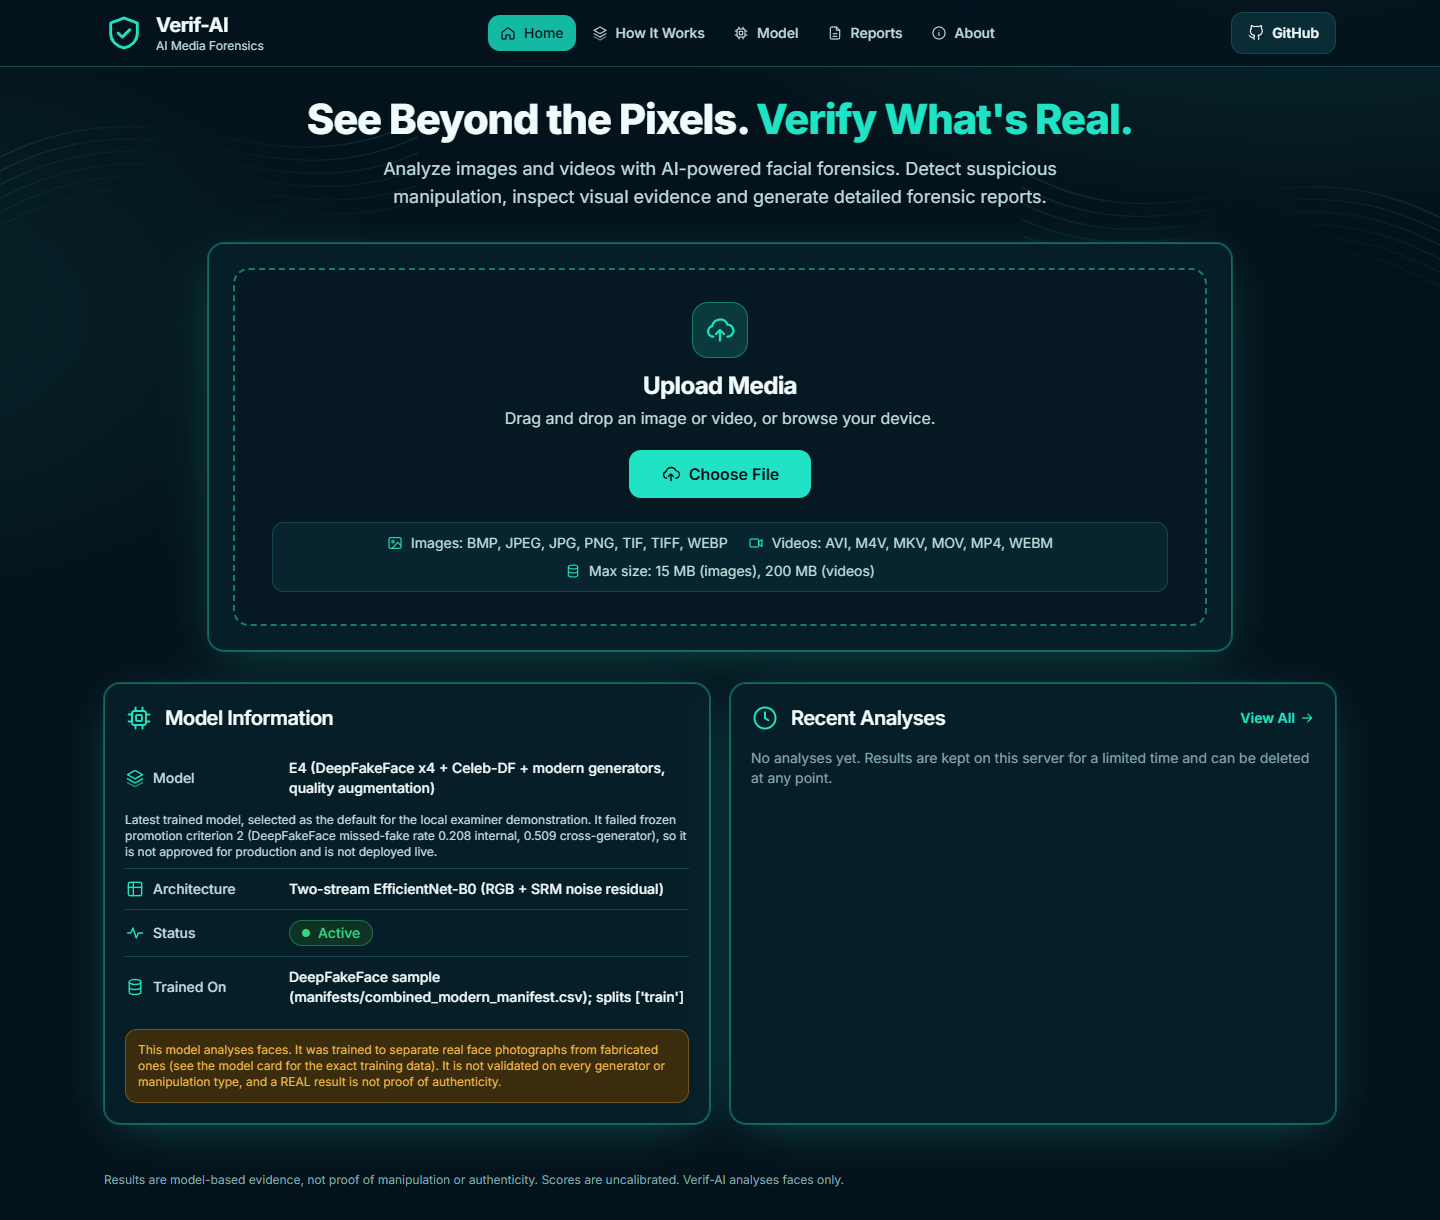
\includegraphics[width=0.6\linewidth]{screenshots/01_home.png}
\caption[Home page of the dashboard (current dark interface; screenshot taken from the running]{Home page of the dashboard (current dark interface; screenshot taken from the running application with an empty history).}
\label{fig:ui-home}
\end{figure}

\subsection{Deployment Architecture}
\label{sec:deploy-design}
The public demonstration separates a static frontend from a hosted API (Figure~\ref{fig:deploy}). The frontend is a build of the React
application served by Vercel; it reads the API address from a build-time environment variable. The API runs in a Docker container on
Render and answers browser requests only for the configured frontend origin (CORS). Results are written to the container's disk, which on the free
tier is not persistent. A paid instance with at least 2\,GB of memory and a disk would be required to run the full model with heat-maps and
durable results.

\begin{figure}[ht]
\centering
\begin{adjustbox}{max width=0.85\linewidth,center}
\begin{tikzpicture}[font=\footnotesize,
  n/.style={draw,rounded corners=3pt,minimum height=1.1cm,align=center,fill=white},
  arr/.style={-{Stealth[length=1.8mm]},thick}]
\node[n,fill=navy!8] (b) at (0,0) {Browser};
\node[n,fill=accent!10,minimum width=3.0cm] (v) at (4.3,0) {Vercel\\static React build};
\node[n,fill=accent!10,minimum width=3.4cm] (r) at (9.2,0) {Render web service\\(Docker, FastAPI + PyTorch)};
\node[n,fill=black!6,minimum width=3.4cm] (d) at (9.2,-2.0) {Instance disk\\(ephemeral on the free tier)};
\draw[arr,<->] (b)--node[above,font=\scriptsize]{page}(v);
\draw[arr,<->] (b.south)--++(0,-1.4)-|node[near start,below,font=\scriptsize]{API calls (CORS: Vercel origin only)}(r.south west);
\draw[arr] (r)--(d);
\end{tikzpicture}
\end{adjustbox}
\caption[Deployment architecture of the public demonstration]{Deployment architecture of the public demonstration. No uploaded media is sent to any service other than the API.}
\label{fig:deploy}
\end{figure}
